\chapter{Results}
\label{cpt:results}


\section{Cache Management Evaluation}
\label{sec:results:cache_partition}

This section describes an experiment that will compare the various implemented cache partitioning algorithms both against \gls{lru} and against each other.
When executing this experiment, we utilize the base system configuration as previously detailed in Table~\ref{tbl:processor_model:properties}.
The L2 cache size is set to 128kB per core, and the L3 cache size is set to 4MB, 8MB or 16MB for respectively 4-, 8- and 16-core workloads.
Each workload is simulated until all benchmarks in that workload have completed at least once. 
The first time a benchmark completes we store its statistics.
After completion, a benchmark will be restarted unless it is the last benchmark to complete in which case we end the workload.
We generate reference statistics for each benchmark by executing it in private mode.
In private mode, we use the same system as in this experiment but with only a single core, the L2 and L3 sizes are set equal to the 4-core workloads; 128kB L2 and 4MB L3.

\begin{figure}[th]
    \centering
    \begin{subfigure}[b]{0.5\textwidth}
        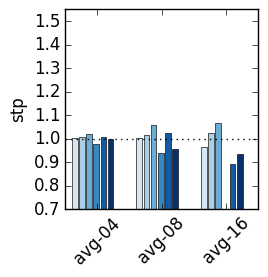
\includegraphics[width=.8\textwidth]{figures/results/speedup/avg-stp-0128k-0100-avg}
        \caption{STP (not shown; PIPP 0.55).}
        \label{fig:results:base:avg:stp}
    \end{subfigure}%
    \begin{subfigure}[b]{0.5\textwidth}
        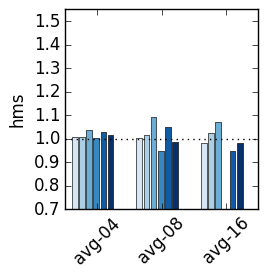
\includegraphics[width=.8\textwidth]{figures/results/speedup/avg-hms-0128k-0100-avg}
        \caption{HMS (not shown; PIPP 0.61).}
        \label{fig:results:base:avg:hms}
    \end{subfigure}
    \begin{subfigure}[b]{0.5\textwidth}
        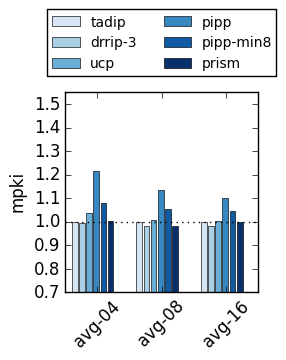
\includegraphics[width=.8\textwidth]{figures/results/speedup/avg-mpki-0128k-0100-avg}
        \caption{MPKI}
        \label{fig:results:base:avg:mpki}
    \end{subfigure}
    \caption[Average result grouped by core]{Average STP, HMS and MPKI normalized to \gls{lru} for all workloads, grouped by number of cores.}
    \label{fig:results:base:avg}
\end{figure}



Figure~\ref{fig:results:base:avg:stp} shows the average speedup of all workloads normalized to \gls{lru} performance grouped by workload size.
We observe that most of the implemented algorithms perform close to \gls{lru} for the four core workloads.
UCP gives the best speedup of 2.1\% while PIPP performs badly with a 2.4\% performance decrease. 
The modified version of PIPP, PIPP-min8, performs as good as \gls{lru}.
When considering the harmonic mean of speedups as shown in Figure~\ref{fig:results:base:avg:hms} we observe that all algorithms perform as good or better than \gls{lru}.  
Most noticeable is PIPP, which in terms of HMS is equal to \gls{lru}.
As explained in Section~\ref{sec:methodology:metrics}, STP  is a measure of the overall speedup of all benchmarks in the workload, and a decrease indicates that completing all of them is slower.
HMS, however, measures the average speedup of each benchmark.
Because PIPP is as good as \gls{lru} measured in HMS, it would indicate that individual benchmarks on average runs equal under PIPP and \gls{lru}.
Figure~\ref{fig:results:base:avg:mpki} shows L3 cache misses, and as expected there is a significant increase, 20\%, in misses for PIPP compared to \gls{lru}, which explains the bad performance. 
The modified PIPP algorithm has a lower increase of 6.7\%.
UCP, which is the highest performer in terms of STP and HMS, gives the third highest miss increase at 3.2\% more misses than \gls{lru}. 

The increase in both misses and performance for UCP could be an artifact of the lookahead algorithm, as shown in detail in Section~\ref{sec:algorithms:ucp}.
If there is a core, which has relatively few cache accesses per allocation period and also only accesses a small number of different blocks.
Then, this core will have a high initial marginal utility as only a few ways are needed to provide hits for most accesses.
Then on the other side of the spectrum there might be a core with many accesses, spread across all cache ways.
This core, which causes more misses in total than the first one, may still have a lower initial marginal utility.
If this is the case, UCP will first allocate ways to cache all the blocks accesses by the first core, before allocating any to the other.
On the other hand, \gls{lru} would have prioritized the second core because it has a higher access frequency.
By shielding the blocks of the first core UCP saves all misses caused by this core, but the other core will miss more compared to the \gls{lru} case.
In total UCP might cause more misses than \gls{lru}.
The overall speedup might, however, be positive if the first core gains more from having fewer misses than the other core loses from having more.


\begin{figure}[th]
    \centering
    \begin{subfigure}[b]{0.5\textwidth}
        \includegraphics[width=\textwidth]{figures/results/speedup/avg-stp-0128k-0100-4-avg}
        \caption{STP}
        \label{fig:results:base:4-avg:stp}
    \end{subfigure}%
    \begin{subfigure}[b]{0.5\textwidth}
        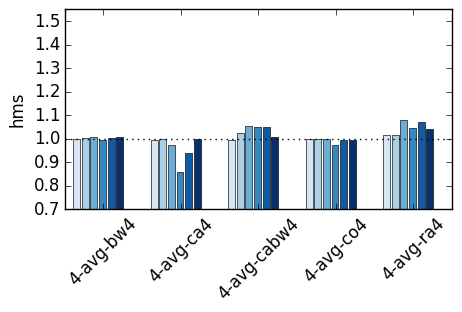
\includegraphics[width=\textwidth]{figures/results/speedup/avg-hms-0128k-0100-4-avg}
        \caption{HMS}
        \label{fig:results:base:4-avg:hms}
    \end{subfigure}
    \begin{subfigure}[b]{0.5\textwidth}
        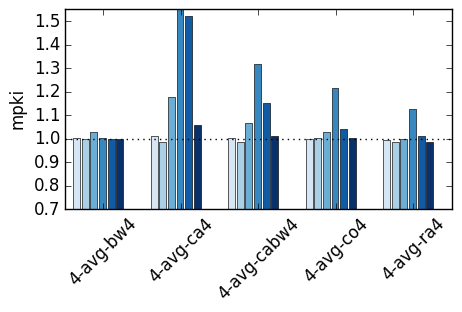
\includegraphics[width=\textwidth]{figures/results/speedup/avg-mpki-0128k-0100-4-avg}
        \caption{MPKI (not shown ca4 pipp 1.9)}
        \label{fig:results:base:4-avg:mpki}
    \end{subfigure}
    \caption[Average result for 4-core workloads]{Average STP, HMS and MPKI normalized to \gls{lru} for all 4-core workload groups.}
    \label{fig:results:base:4-avg} 
\end{figure}


With increasing core count, we increase the size of the L3 cache, but the associativity is unchanged.
As a result, even more cores have to share the 32 blocks in each cache set.
For some algorithms, especially PIPP, this increased cache set pressure significantly degrades performance.
At 8-cores, PIPP has a 7.2\% performance decrease measured in STP compared to \gls{lru}.
The modified PIPP-min8 outperforms PIPP, and even slightly outperforms \gls{lru} by 2.2\%, in the same situation.
This is an indication that blocks inserted by PIPP do not stay in the cache for long enough to see much re-use.
The modified algorithm seems to counteract this problem by inserting with an offset of 8 blocks higher than normal PIPP.
In the 16-core case, this effect is even more visible, with PIPP performing 45\% worse than \gls{lru} measured in STP and PIPP-min8 at only 7.6\% worse than \gls{lru}.
DRRIP and UCP, the two best performers in the 4-core case, continue to perform well for both 8- and 16-cores.
UCP beating \gls{lru} by 5.7\% and 6.9\% measured in STP in 8- and 16-core workloads, and DRRIP at 1.8\% and 2.6\%.
TADIP and PriSM, which both perform equal to \gls{lru} in the 4-core case, lose some traction when core count increases.
TADIP performs equal to \gls{lru} for 8-cores, but 3.6\% slower for 16-cores.
PriSM cannot keep up for more than 4-cores, and performs 4.7\% and 7.6\% slower for 8- and 16-cores.
As the number of cores increase, it might be tempting to blame TADIP's performance loss on an increased fraction of duel-sets, more duel-sets means more sets forced to use a non-optimal policy.
However, since we scale the shared cache size linearly with increased core count while keeping the associativity static, the number of sets increase with the core count.
Hence, the fraction of duel sets is equal in all cases.
Neither TADIP nor PriSM caused an increase in misses, which is a good result considering they target miss-minimization.
The fact that UCP can increase STP while increasing misses, and TADIP and PriSM decreases STP without affecting miss count is an important result that shows that miss minimization does not directly imply a speedup.

Our 4-core workloads consist of five distinct groups, where four of the groups contain benchmarks with a specific characteristic.
Section~\ref{sec:methodology:benchmarks} lists each group and explain their specific characteristics.
Figure~\ref{fig:results:base:4-avg} shows average STP, HMS and MPKI normalized to \gls{lru} for these five groups.
Exploring the result from each of these groups individually is useful as it will show how various algorithms react to specific workload characteristics.

Bandwidth bound workloads contain benchmarks that do not benefit from increased cache space.
These are benchmarks with mainly streaming access patterns. 
As expected the results show that none of the algorithms can significantly improve performance compared to \gls{lru}.
As seen in Figure~\ref{fig:results:base:4-avg:mpki} UCP causes 3\% more misses than \gls{lru}, and in return increases STP by 4.8\% compared to \gls{lru}.
We expect that even our bandwidth bound benchmarks will have phases with memory re-references, which means that their utility will increase.
Based on our results, UCP seems to detect these phases and prioritize benchmarks correctly.
While PIPP in theory also should be able to detect such changes, our result shows it does not.
A possible explanation to this is that PIPP uses both utility and streaming flags.
While an application may periodically have increased utility causing UCP to prioritize it, PIPP might still consider it as streaming due to a high miss-fraction, if this is the case, PIPP will ignore the increased utility.

Cache bound workloads contain benchmarks that are sensitive to changes in available cache space.
In general these benchmarks have recency-friendly access patterns.
Our results from these workloads show two main trends.
First, as expected, \gls{lru} performs well, and none of the other algorithms increases performance or significantly reduce misses.
Secondly, UCP and PIPP, the two algorithms that perform way partitioning, both reduce performance and cause a significant miss increase. 
While TADIP and DRRIP, which both mimic \gls{lru} and PriSM, which performs a variant of block level partitioning, performs as good as \gls{lru} in terms of performance.
From this, we see that way partitioning is not beneficial if all benchmarks are recency-friendly.
This is an expected result, as way-partitioning is designed to improve performance by shielding recency-friendly access patterns from thrashing caused by other cores.
When all applications are recency-friendly, it seems that having the cores dynamically share the cache based on access frequency is a better solution.
PriSM, which does block level partitioning, confirms this assumption as it performs as good as \gls{lru} in terms of STP and HMS.
It does, however, cause a small increase in misses.


\begin{figure}[th]
    \centering
    \begin{subfigure}[b]{0.5\textwidth}
        \includegraphics[width=\textwidth]{figures/results/speedup/speedup-stp-0128k-0100-cabw4}
        \caption{STP}
        \label{fig:results:base:cabw:stp}
    \end{subfigure}%
    \begin{subfigure}[b]{0.5\textwidth}
        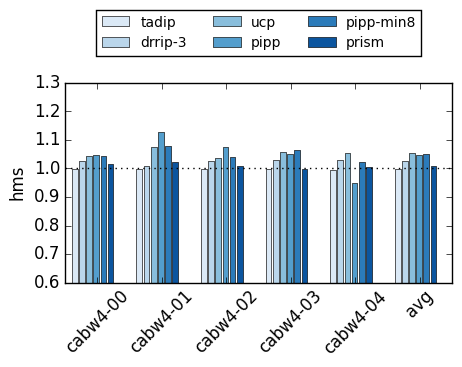
\includegraphics[width=\textwidth]{figures/results/speedup/speedup-hms-0128k-0100-cabw4}
        \caption{MPKI}
        \label{fig:results:base:cabw:mpki}
    \end{subfigure}
    \caption[cabw workloads result]{STP and MPKI normalized to \gls{lru} for cache and bandwidth bound workloads.}
    \label{fig:results:base:cabw} 
\end{figure}

The performance of compute-bound workloads is expected to be mostly unaffected by the partitioning algorithm. 
Our results support this assumption, with the exception of PIPP, which again causes increased misses and a slight performance decrease.
Once again, PIPP-min8 seems to remedy this, pointing to an issue with short block lifetimes in a PIPP managed cache, causing more misses.

Both cache and bandwidth bound workloads and the random workloads show results that concur with the overall averages discussed earlier.
One interesting fact to note is that both versions of PIPP and UCP are equally good and also the best performers when measuring in HMS in cache and bandwidth bound workloads.
This result points to PIPP being able to provide speedups of individual benchmarks that are good enough to raise the average while still performing as good as \gls{lru} measured in STP.
Most likely this indicates that applications marked as streaming are performing badly while those shielded are performing so good their performance increase raises the average.


In all our previous findings, we have observed that UCP is raising performance while also increasing misses.
To ensure that this result is not just an artifact of result averaging, we show the per workload STP and MPKI for the cache and bandwidth bound workloads in Figure~\ref{fig:results:base:cabw}.
As expected, the STP measurements show UCP providing a speedup in four out of five workloads.
In the fifth workload, cabw01, UCP performs as good as \gls{lru}.
When considering the MPKI measurements, we observe that UCP increase misses by at least 30\% in the four workloads where performance is best.
We also note that in the case where UCP performs as good as \gls{lru}, it also causes the least number of misses.
These same trends are also visible in our other results.
Based on this, we conclude that UCP can increase performance while also increasing misses.


\chapter{Sensitivity Analysis}
\label{cpt:sresults}
This chapter outlines a total of five experiments exploring the sensitivity of our simulated system and our cache partitioning results to various changes in the simulated architecture.
The first experiment, covered in Section~\ref{sec:results:model_sensitivity}, will investigate the stability of our processor model and attempt to uncover and remove any bottlenecks.
Then Section~\ref{sec:results:csmb_sensitivity} explores how simulation clock skew in Sniper affects the outcome of our experiments.
Sections~\ref{sec:results:l2size_sensitivity} and~\ref{sec:results:l3size_sensitivity} explore how algorithm performance is affected by the size of the L2 and L3 cache respectively.
Finally, Section~\ref{sec:results:bus_sensitivity} explores how changing the bandwidth of the memory controller affects algorithm performance.



\section{Processor Model Parameter Sensitivity}
\label{sec:results:model_sensitivity}

As detailed in the processor model overview, in Section~\ref{sec:methodology:processor_model}, we have based our simulated processor core on the Nehalem~\cite{Thomadakis2011} architecture.
An experiment was devised, with the goal of gaining a better understanding and improved confidence in this model.
Of the properties used to define the model, we selected a total of five we believe to have an important impact on the performance of the simulated core.
We then varied each of the properties in isolation, keeping the others constant.
For each parameter combination, we ran all our benchmarks and calculated the average speedup relative to the base configuration.
The result of this experiment will show us how sensitive our simulated core is to configuration changes.
If we observe a significant performance variation when changing one or more of the selected properties, we might have uncovered a bottleneck.
In this case, it might be necessary to tweak the model until we find one that is less sensitive to change.

\begin{figure}[H]
        \centering
        \begin{subfigure}[b]{0.5\textwidth}
                \includegraphics[width=\textwidth]{figures/processor_model/ol}
                \caption{Outstanding Loads.}
                \label{fig:results:processor_model:ol}
        \end{subfigure}%
        \begin{subfigure}[b]{0.5\textwidth}
                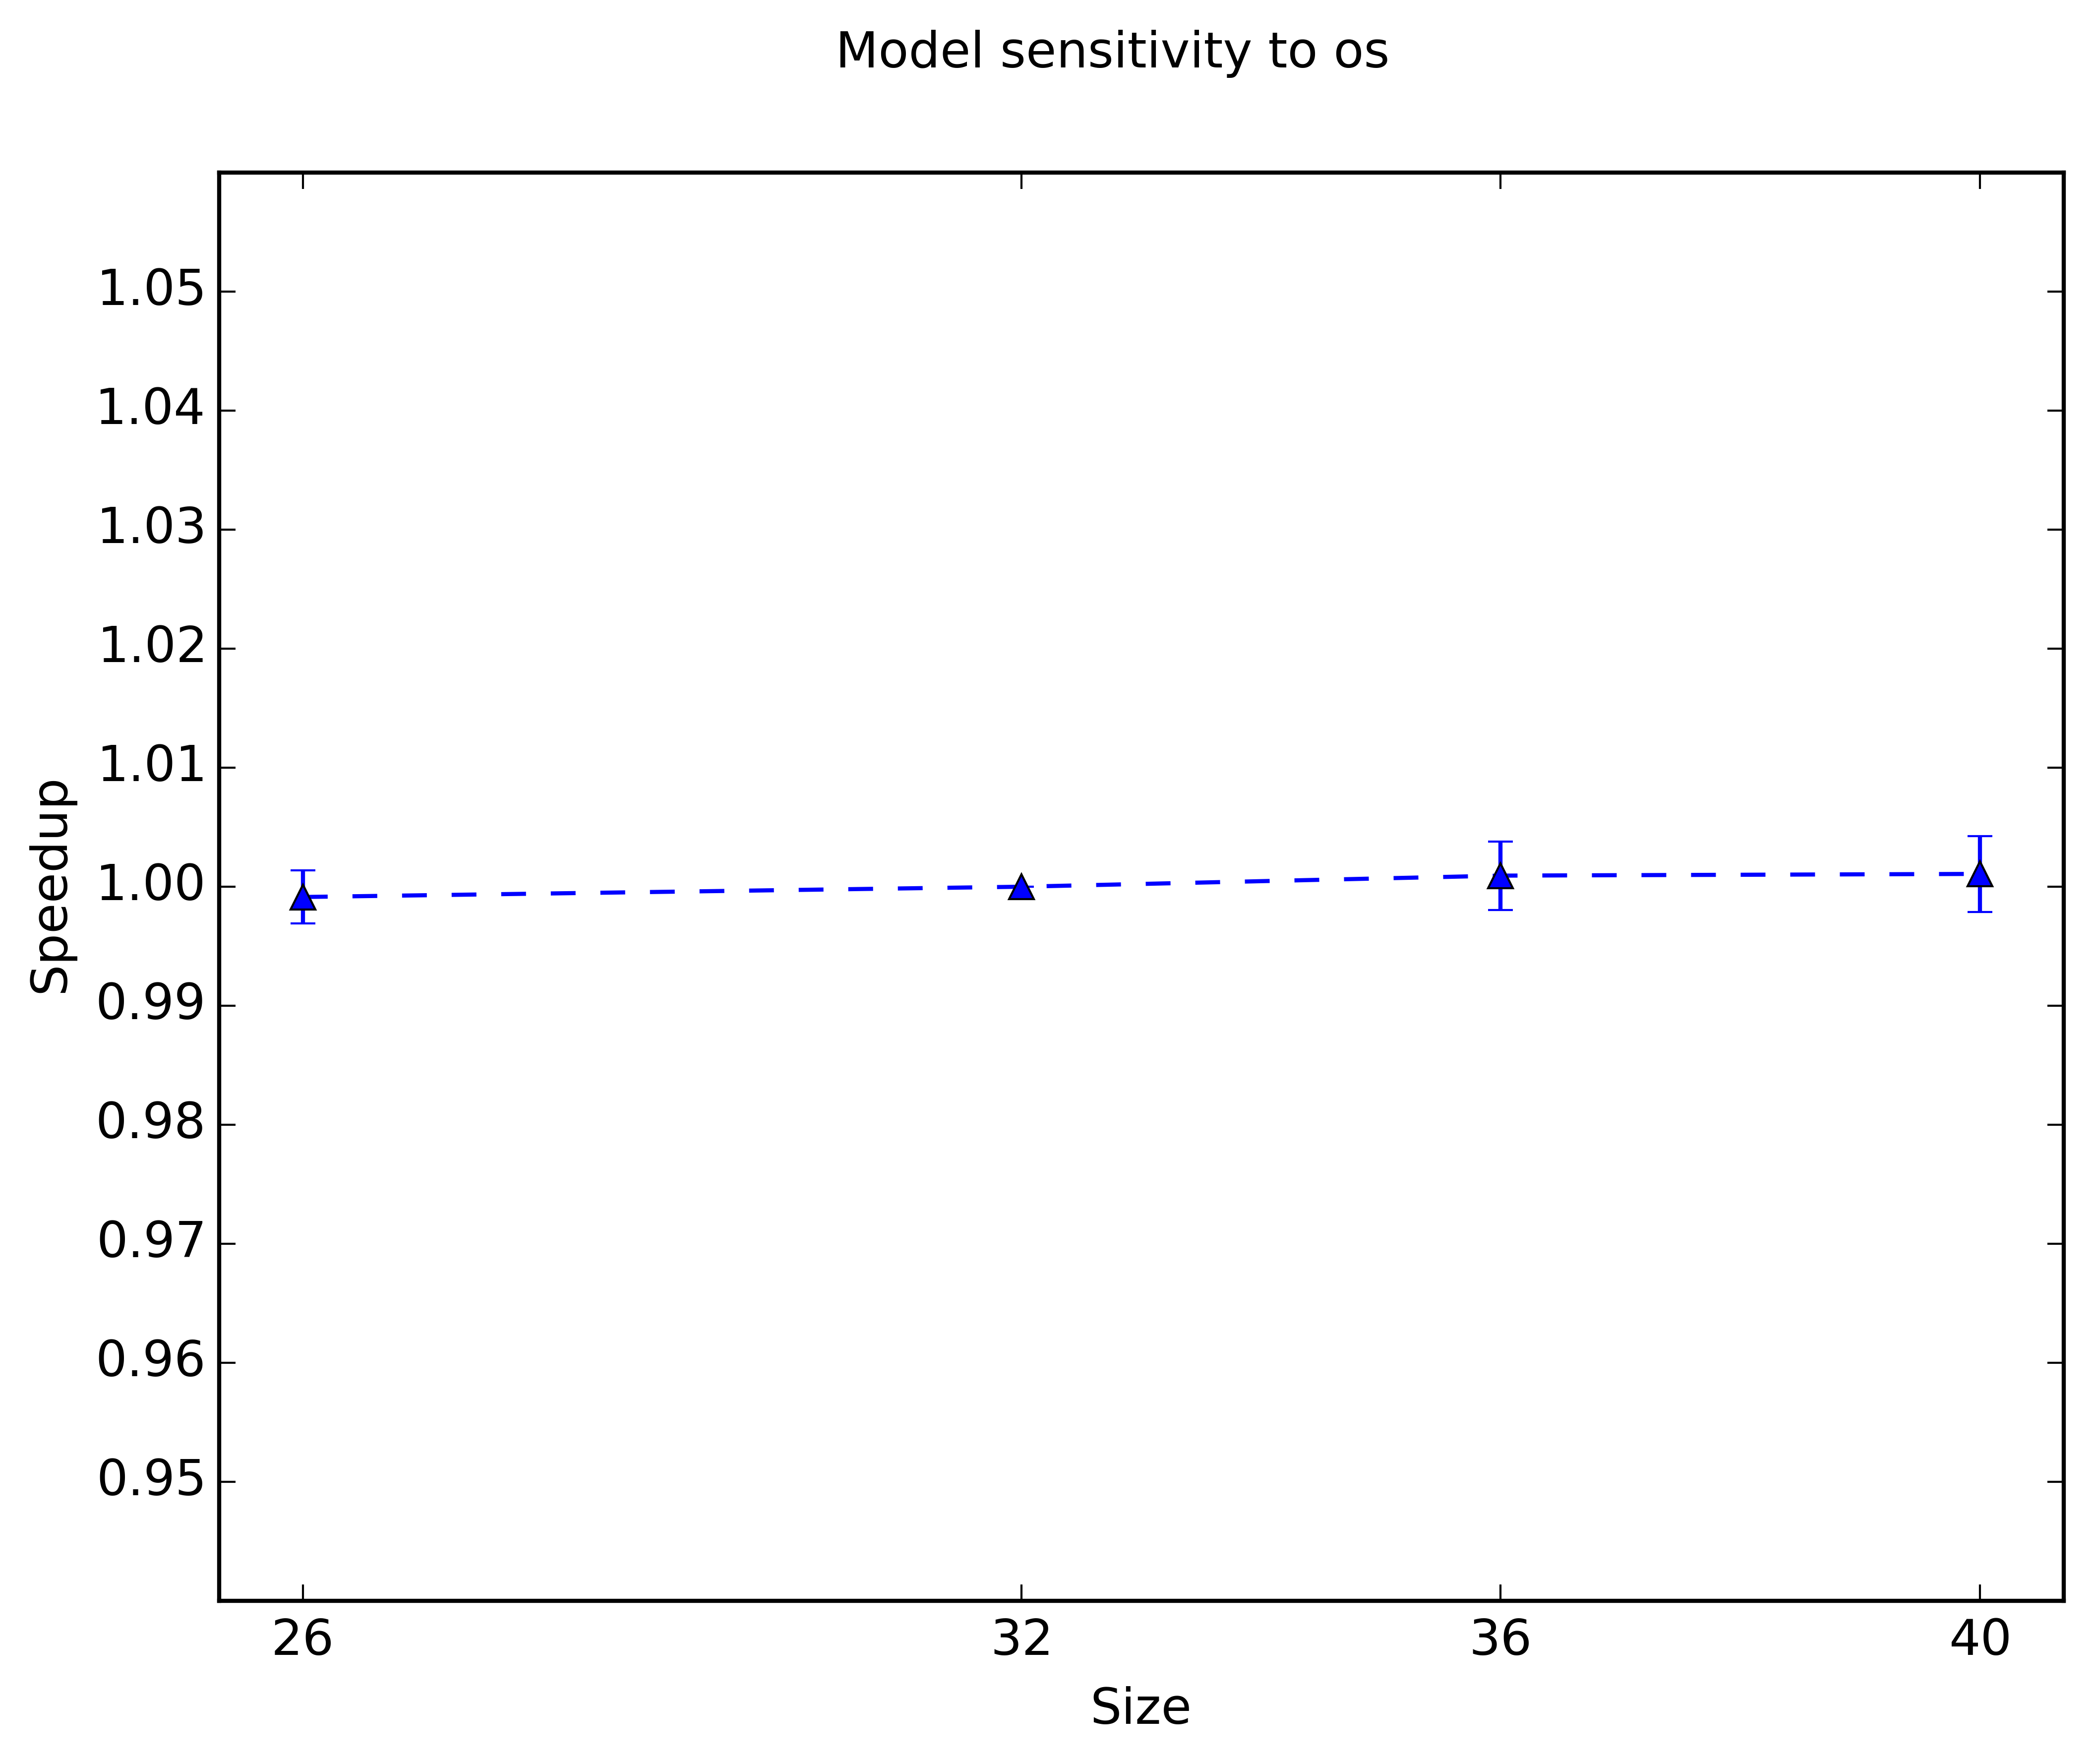
\includegraphics[width=\textwidth]{figures/processor_model/os}
                \caption{Outstanding Stores.}
                \label{fig:results:processor_model:os}
        \end{subfigure}
        \begin{subfigure}[b]{0.5\textwidth}
                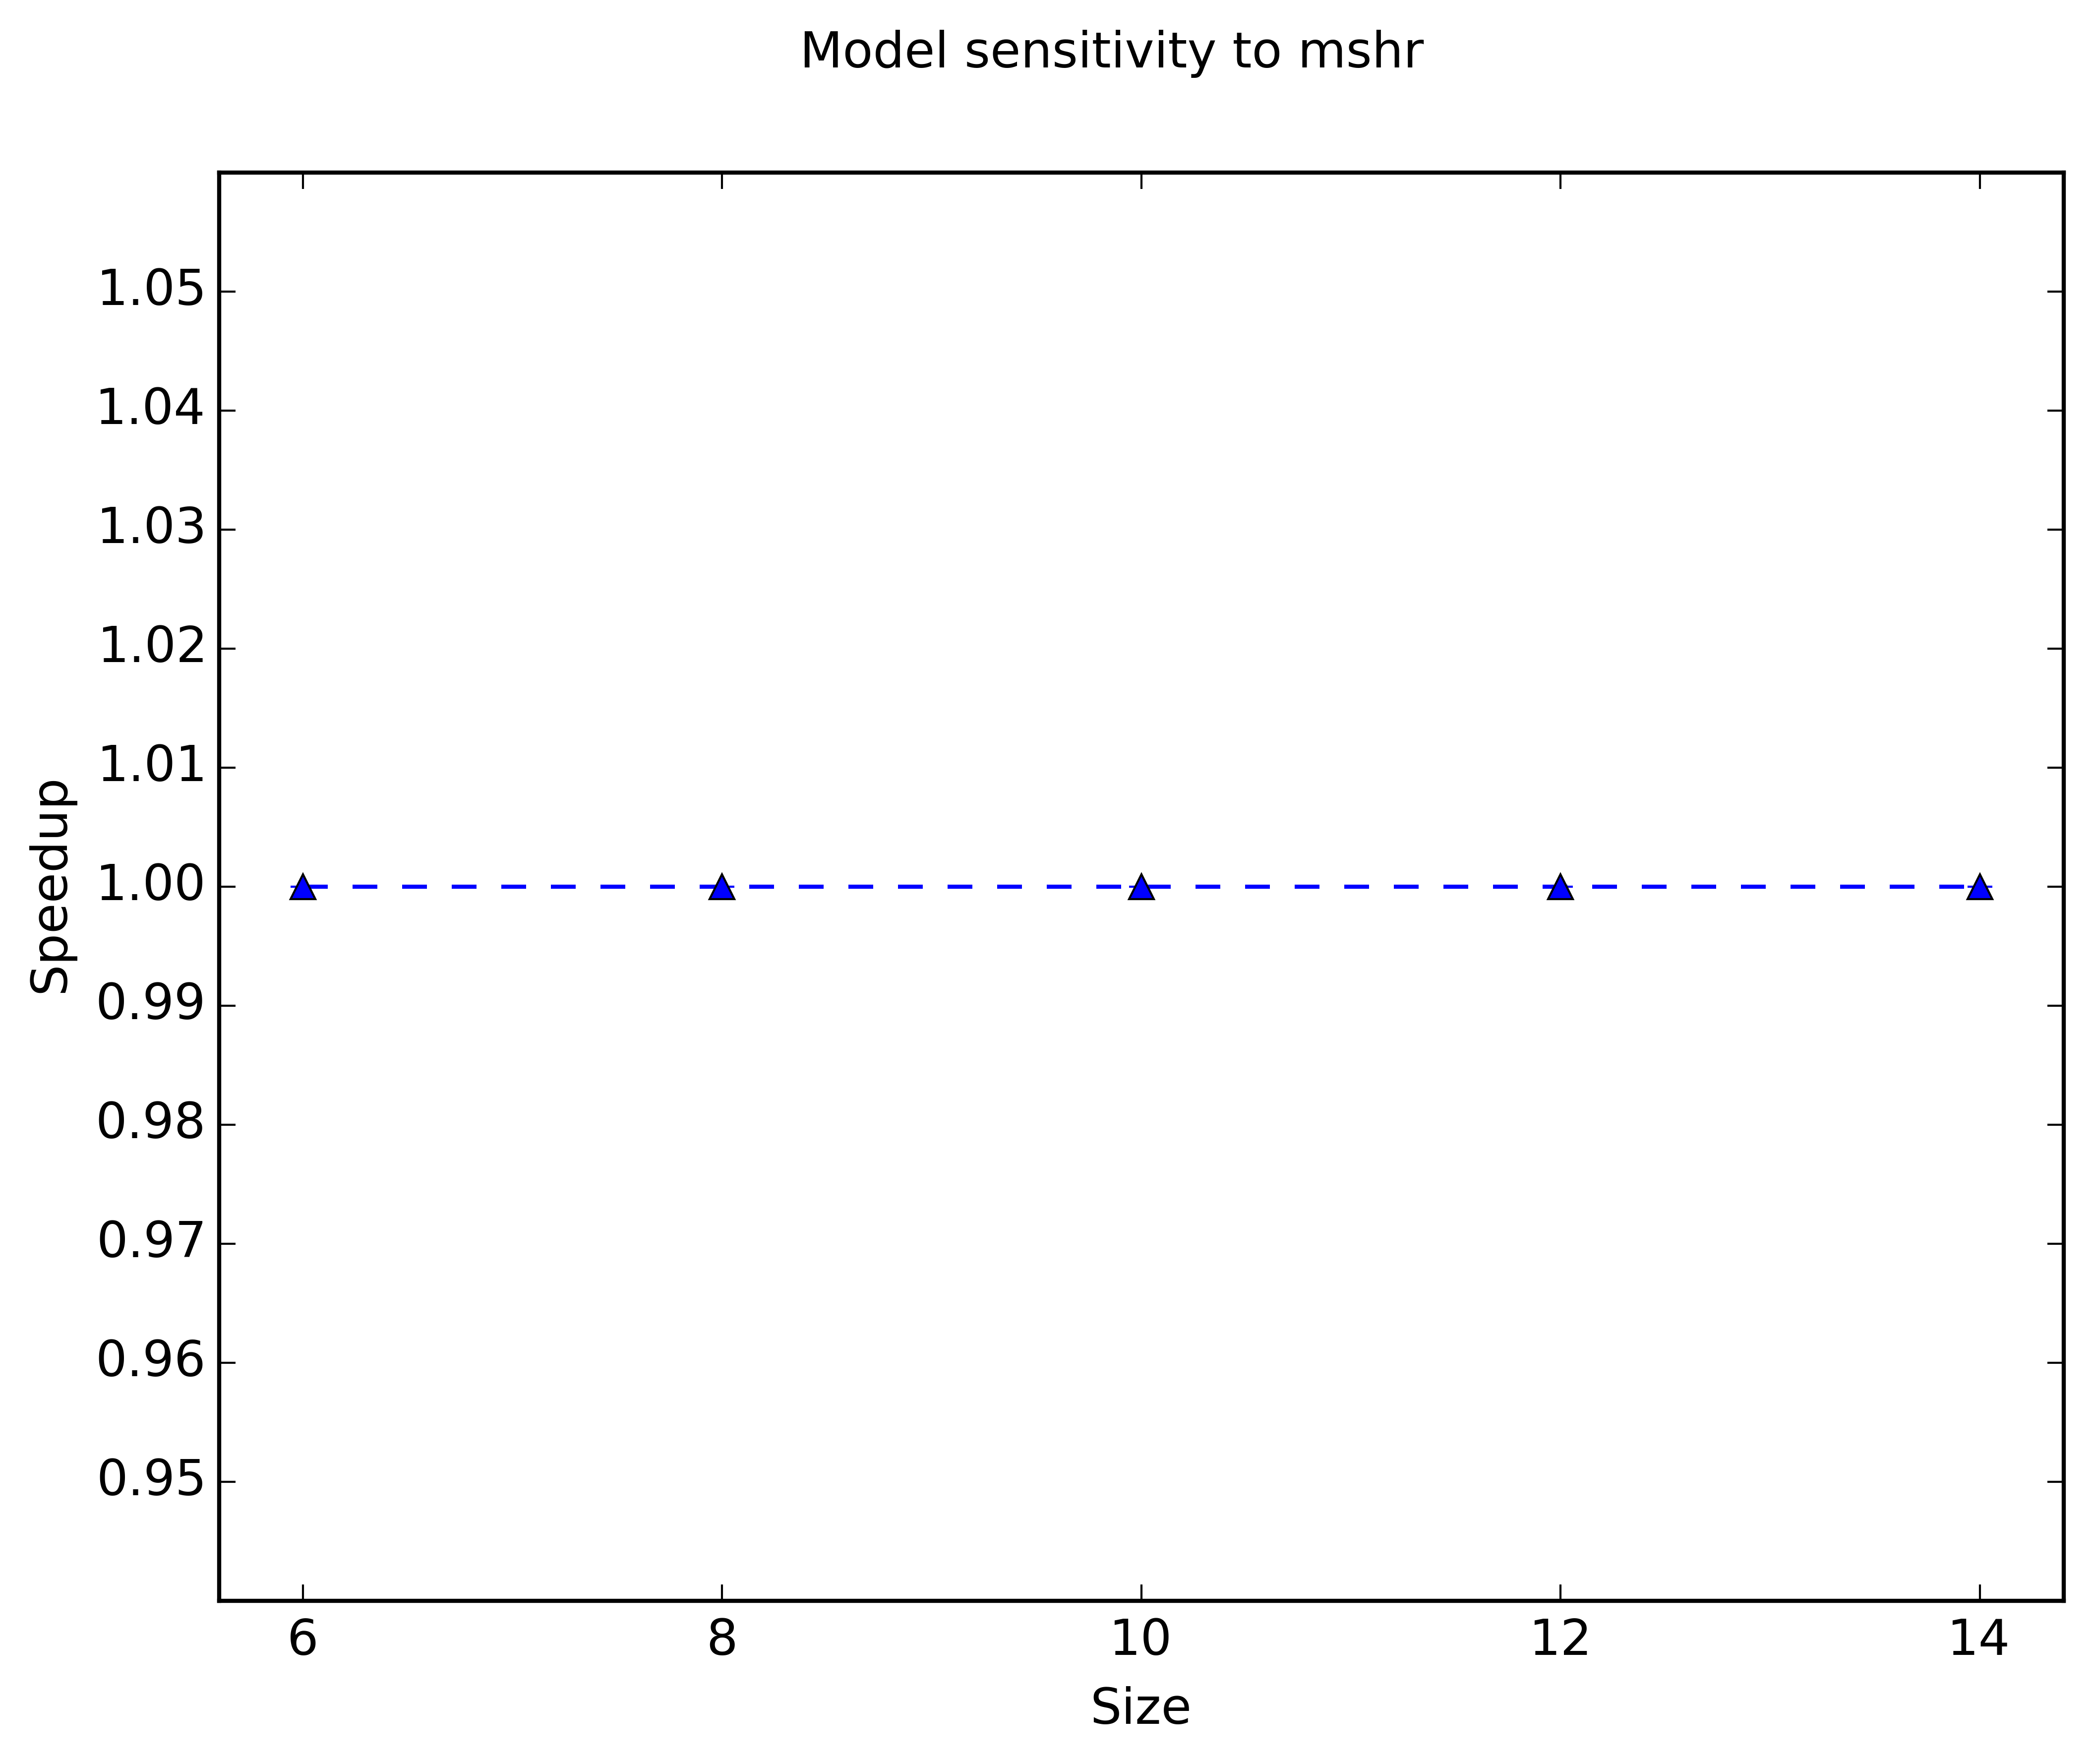
\includegraphics[width=\textwidth]{figures/processor_model/mshr}
                \caption{L1 Miss Status Hold Register.}
                \label{fig:results:processor_model:mshr}
        \end{subfigure}%
        \begin{subfigure}[b]{0.5\textwidth}
                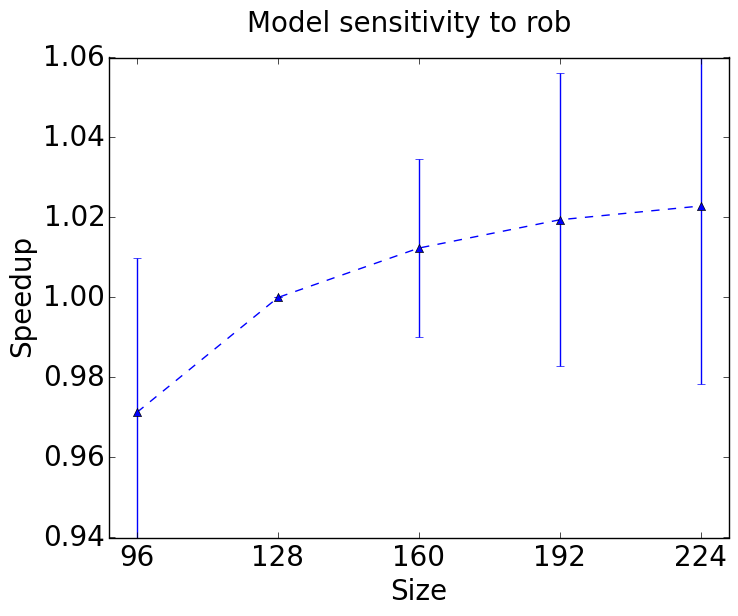
\includegraphics[width=\textwidth]{figures/processor_model/rob}
                \caption{Re-order Buffer.}
                \label{fig:results:processor_model:rob}
        \end{subfigure}
        \begin{subfigure}[b]{0.5\textwidth}
                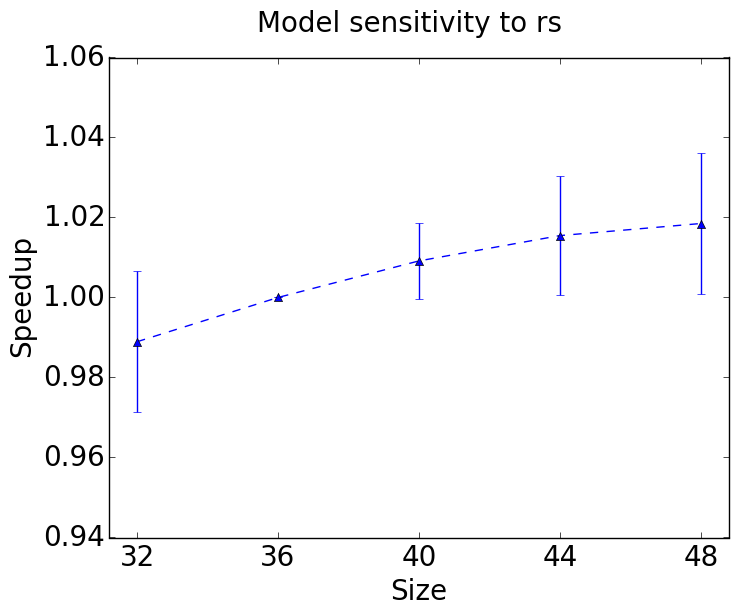
\includegraphics[width=\textwidth]{figures/processor_model/rs}
                \caption{Reservation Station.}
                \label{fig:results:processor_model:rs}
        \end{subfigure}%
        \caption{Core model property sensitivity.}
        \label{fig:results:processor_model}
       ~ % Fill page, prevents latex from placing a single line of text under the figure
\end{figure}

Figure~\ref{fig:results:processor_model} shows the average speedup of all benchmarks when we vary our five selected properties; Outstanding loads (ol), outstanding stores (os), L1 miss status holding registers (MSHR), re-order buffer size (rob) and reservation station entries (rs).
Outstanding loads and stores specify the number of outstanding memory requests the core can have active in the rob.
The number of L1 MSHRs decide how many outstanding cache misses the first level cache can handle before it has to block on a miss.
The size of the rob and rs together decide how many instructions can be live during execution.  
Increasing the number of live instructions can increase the amount of \gls{ilp} the processor can extract from the program while possibly increasing the cost of a branch miss prediction.

For two of the memory related properties; os and ol, we observe no improvement nor decrease in performance for the values we explored.
When we increase the last memory related parameter, MSHR, we do observe a slight performance change.
With an increasing number of MSHRs, the cache and hence the core can handle more outstanding memory requests. 
As a result, the core will be able to exploit more \gls{ilp}, and a slight performance improvement is observed. 
Unlike the MSHRs, we do not expect the value of os and ol to affect performance. 
If the core is to gain performance from supporting more outstanding loads there has to be more than 48 loads among the 128 instructions that fit in the rob. 
Equally there must be more than 32 stores per 128 instructions for an increased os limit to be beneficial.
Also, both os and ol are limited by the number of memory requests the memory system can handle, and the total number of L1 MSHRs is less than the size of both os and ol.
The observed performance gain when increasing the number of MSHRs in the first level caches, as seen in Figure~\ref{fig:results:processor_model:mshr}, is less than 1\% with a 50\% storage increase. 
We also observe a standard deviation of more than 3\%. 

When Increasing the size of the rob and the number of rs entries, we observe a slight increase in performance.
Figures~\ref{fig:results:processor_model:rob}~and~\ref{fig:results:processor_model:rs} show an average performance increase of about 2\% with more rob entries, and about a 3\% increase with more rs entries.
We observe that these increases come at the cost of a 75\% and 50\% storage increase respectively.
Also, we observe that the standard deviation in both cases is about the same as the average performance increase.

When reviewed, these results lead us to conclude that the processor model we have presented, based on the Nehalem architecture, is stable and that we have no obvious performance gains from small adjustments.
As a result, we decide to continue using this model for the rest of our experiments without making any adjustments.

Considering that we base our model on an actual architecture and that our simulator strives to simulate the core model of that same architecture, it is not a far-fetched result observing little sensitivity to property changes.
During the design process of the architecture, it is natural to expect that the designers made a conscious choice between speed and area using a similar analysis.
The final properties would then most likely have been selected to provide a stable middle ground, which we see reflected in our simulation results.

\section{Clock Skew Sensitivity}
\label{sec:results:csmb_sensitivity}

As explained in section~\ref{sec:framework:simulator} one of the techniques that make Sniper faster than conventional cycle-accurate simulators, such as gem5, is the use of multiple simulation threads that each simulate one processor core.
A method that keeps the simulation threads in sync is required to simulate inter-core interactions correctly.
The method used to keep the threads in sync affects both simulation accuracy and simulation time.
By having a relaxed synchronization method, one can improve simulation time, at the cost of simulation accuracy.
In our experiments, we have used barrier synchronization with a barrier width of 100 cycles.
Any inter-core interactions that occur between two successive barriers are not guaranteed to occur in the correct order, but events separated by a barrier will be simulated in the correct order.
In other words, within a single barrier there is the possibility that all simulation threads run sequentially.
For our work, this implies that there is a possibility that memory requests within a barrier arrives in the cache sorted by the core id, and not by time.
Because of this possibility we expect that changing the clock skew minimization barrier (CSMB) value could have a noticeable effect on our experimentation results.

\begin{figure}[th]
    \centering
    \begin{subfigure}[b]{0.5\textwidth}
        \includegraphics[width=0.8\textwidth]{figures/results/speedup/csmb-stp-0128k-0100-csmb-4}
        \caption{STP sensitivity to CSMB.}
        \label{fig:results:csmb:stp}
    \end{subfigure}%
    \begin{subfigure}[b]{0.5\textwidth}
        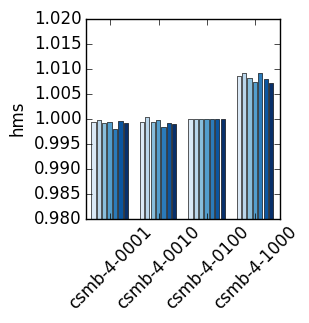
\includegraphics[width=.8\textwidth]{figures/results/speedup/csmb-hms-0128k-0100-csmb-4}
        \caption{HMS sensitivty to CSMB.}
        \label{fig:results:csmb:hms}
    \end{subfigure}
    \begin{subfigure}[b]{0.6\textwidth}
        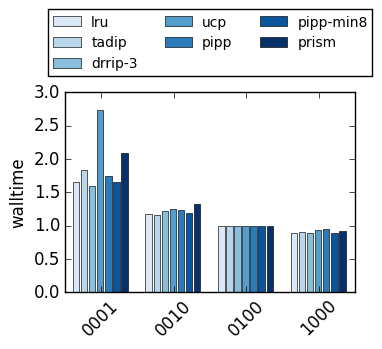
\includegraphics[width=.8\textwidth]{figures/results/speedup/csmb-walltime-0128k-0100-csmb-4}
        \caption{walltime sensitivity to CSMB.}
        \label{fig:results:csmb:walltime}
    \end{subfigure}
    \caption{STP, HMS and walltime sensitivity to size of CSMB.}
    \label{fig:results:csmb}
\end{figure}


We devised an experiment to investigate how much the choice of synchronization barrier width affects our results, and also how much it affects simulation time.
In the experiment, we vary the value of the CSMB and compare average STP, HMS and MPKI values for all 4-core workloads.
Figure~\ref{fig:results:csmb} contains plots for both STP and HMS relative to the default 100 cycle barrier.
From the graph, it is apparent that lowering the value below 100 cycles causes negligible variations in our average results. 
The most noticeable is PIPP; that varies by about 0.2\% with a tighter barrier interval.
Increasing the interval to 1000 cycles results in a more noticeable difference in measurements.
For both HMS, shown in figure~\ref{fig:results:csmb:hms}, and MPKI, not shown, the trends are the same.

The variance in simulation walltime when we vary CSMB values, as shown in figure~\ref{fig:results:csmb:walltime}, is as expected. 
When lowering the barrier interval we measure an increase in average walltime.
Increasing the barrier value causes a slight decrease in walltime.
We observe that the performance gain by increasing the barrier is small compared to the result variation. 
When decreasing the barrier, the opposite is true; the result variation is small compared to the walltime increase.
These observations suggest that a barrier width of 100 cycles is a good trade-off between accuracy and walltime.

\section{L2 Cache Size Sensitivity}
\label{sec:results:l2size_sensitivity}

In this section, we investigate how increasing the size of the private cache affects the performance of the cache partitioning algorithms.
We ran the same experiment as in Section~\ref{sec:results:cache_partition}, but with varying L2 sizes.
The L2 configurations are as shown in Table~\ref{tbl:processor_model:l2}, to summarize we utilize cache sizes of 128kB, 256kB, 512kB, and 1024kB.
As in previous experiments, we set the L3 size depending on the workload size.
In this experiment, we only utilize the three random workload groups.
We do this to be able to aggregate and compare 4-core results to 8- and 16-core results.
We omit the 4-core workloads with specific traits because they would bias the overall 4-core averages.
Also, we have only included plots of the STP results, this because HMS and MPKI results did not add any additional insight in this experiment.

Figure~\ref{fig:results:l2:access} shows the average number of L3 accesses for random workloads with varying L2 cache size.
As can be seen from the graph, by increasing the size of the L2 cache we are decreasing the number of accesses to the L3 cache.
In other words, the L2 caches are hiding an increasing amount of memory requests from the shared level.
We expect this increased filtering of requests to have an impact on the performance of the implemented algorithms.



\begin{figure}[th]
    \centering
    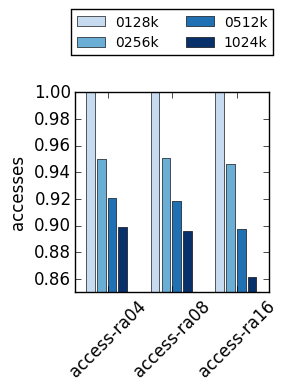
\includegraphics[scale=0.5]{figures/results/speedup/accesses-accesses-0128k-0100-access}
    \caption{Relative number of accesses to L3 cache with varying L2 size.}
    \label{fig:results:l2:access}
\end{figure}

\begin{figure}[!th]
    \centering
    \begin{subfigure}[b]{0.5\textwidth}
        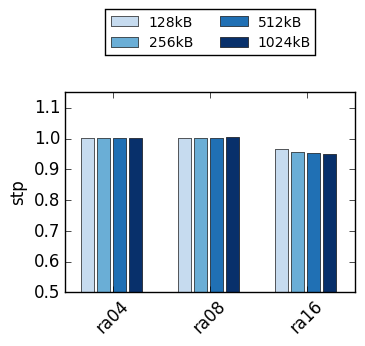
\includegraphics[scale=0.6]{figures/results/speedup/l2-legend-stp-0128k-tadip-l2}
        \caption{Speedup of TADIP normalized to LRU.}
        \label{fig:results:l2:tadip}
    \end{subfigure}%
    \begin{subfigure}[b]{0.5\textwidth}
        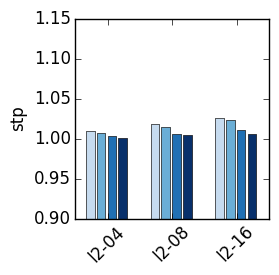
\includegraphics[scale=0.6]{figures/results/speedup/l2-stp-0128k-drrip-3-l2}
        \caption{Speedup of DRRIP normalized to LRU.}
        \label{fig:results:l2:drrip}
    \end{subfigure}
    \begin{subfigure}[b]{0.5\textwidth}
        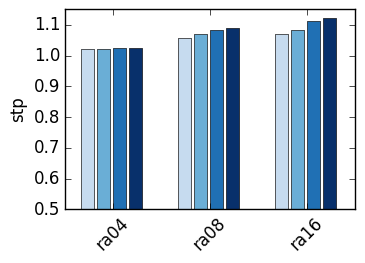
\includegraphics[scale=0.6]{figures/results/speedup/l2-stp-0128k-ucp-l2}
        \caption{Speedup of UCP normalized to LRU.}
        \label{fig:results:l2:ucp}
    \end{subfigure}%
    \begin{subfigure}[b]{0.5\textwidth}
        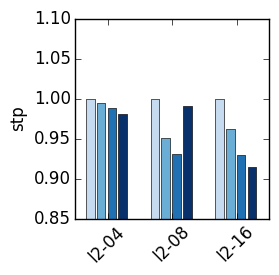
\includegraphics[scale=0.6]{figures/results/speedup/l2-stp-0128k-prism-l2}
        \caption{Speedup of PriSM normalized to LRU.}
        \label{fig:results:l2:prism}
    \end{subfigure}
    \begin{subfigure}[b]{0.5\textwidth}
        \includegraphics[scale=0.6]{figures/results/speedup/l2-stp-0128k-pipp-l2}
        \caption{Speedup of PIPP normalized to LRU.}
        \label{fig:results:l2:pipp}
    \end{subfigure}%
    \begin{subfigure}[b]{0.5\textwidth}
        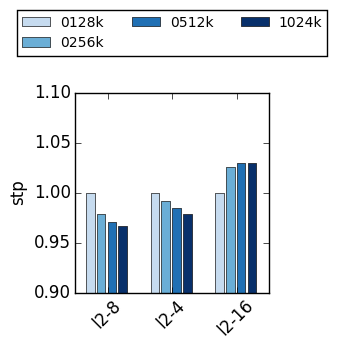
\includegraphics[scale=0.6]{figures/results/speedup/l2-stp-0128k-pipp-min8-l2}
        \caption{Speedup of PIPP-min8 normalized to LRU.}
        \label{fig:results:l2:pipp-min8}
    \end{subfigure}
    \caption[Speedup with increasing L2 size]{Speedup of cache partition algorithms normalized to LRU with increasing private L2 size}
    \label{fig:results:l2}
\end{figure}

Figure~\ref{fig:results:l2:tadip} shows the speedup of TADIP normalized to LRU measured in STP. 
As seen previously, TADIP performs as good as LRU in both 4- and 8-core workloads with a 128kB L2 cache.
With increasing L2 cache size TADIP steadily outperforms LRU with between 0.1\% and 0.6\% depending on the configuration. 
At 16-cores, TADIP underperforms compared to LRU, as previously shown.
We note that, in this case, increasing the L2 size seems to cause a further decrease in TADIP performance, while the opposite is true in the 8-core case.
We expect that TADIP will react slower to changes in application phases as memory filtering increases, because of the counter architecture used to switch between algorithms.
This effect does not seem to have a noticeable impact on results for the 4- and 8-core runs, but we assume it is causing the visible decrease in performance for the 16-core runs.

DRRIP as already covered outperforms LRU, Figure~\ref{fig:results:l2:drrip} confirms this.
The figure also shows that increasing the L2 size causes a reduction in DRRIP performance.
We know that DRRIP uses a step-wise promotion policy where each successive access promotes a block one position.
Naturally less information about successive accesses will be available to the shared level as filtering in the private levels increase.
It is consequently not unexpected that DRRIP suffers from increased filtering by private cache levels.
From the figure, we note that DRRIP seems to be slightly less sensitive to small changes in L2 size with increasing core count, but in all cases a 1024kB L2 causes DRRIP performance to mimic LRU performance.

In contrast to the previous algorithms, UCP performance increases with L2 cache size in all workloads, as seen in Figure~\ref{fig:results:l2:ucp}.
We know that UCP uses a utility algorithm as the mechanism for allocating ways to cores. 
The input to this algorithm changes when we increase filtering of requests to the shared cache level.
As a result, the allocation of ways to cores is also expected to change, but this is the intended mechanism of UCP and should not negatively affect performance.
UCP uses LRU to manage replacement for each core, but UCP under normal circumstances only allows a core to evict one of its own blocks. 
We have already covered that this is why UCP outperforms LRU in the base configuration, in Section~\ref{sec:results:cache_partition}. 
As filtering increases at the private level, we notice that UCP increases its performance compared to LRU. 
We expect that this is because, with increased private cache, more requests from recency-friendly applications can be satisfied by the private levels and less information reaches the shared level.
Trashing and streaming applications will still have its requests propagate to the shared cache, largely independent of the size of the private cache. 
Hence with increasing private cache size we expect LRU to make worse decisions by prioritizing trashing and streaming patterns due to their access frequency.
UCP with utility-based way-partitioning will not suffer as much from the lack of information about recency-friendly applications, and as the results state, can take advantage of increasing private cache size.

PriSM calculates target allocations for each core with the goal of reducing misses.
This technique bears some resemblance to the utility calculation done by the UMON.
As with UCP, we expect PriSM to be able to increase its performance compared to LRU with increased private cache size because it will continue to limit the cache use of streaming and trashing applications.
We find this expectation reflected in our results.
For both 4- and 16-core workloads we observe an increase in performance compared to LRU as the size of private cache increases.
In the 8-core results we see the same trend between the smallest and largest L2 configuration, but we unexpectedly observe a performance drop for 256kB and 512kB configurations. 
It is unclear what causes this performance drop, and further work is required to analyze this.

Finally Figure~\ref{fig:results:l2:pipp} show the performance of PIPP, and Figure~\ref{fig:results:l2:pipp-min8} shows the performance of the modified PIPP algorithm.
Since PIPP uses the same utility algorithm as UCP and also aims to achieve the same allocations as UCP, we expect them to show similar trends.
This expectation somewhat holds true for the 4-core case, where there is a slight upward trend with increasing L2 size.
However, PIPP underperforms compared to LRU in all workloads, and with increasing core count performance drops significantly.
We expect the short lifetime of blocks in PIPP managed caches to be the cause of this, as covered in Section~\ref{sec:results:cache_partition}.
The modified PIPP algorithm shows a performance development much closer to what is expected, at least for 4- and 8-core workloads.
We observe the same increase in performance with increased L2 cache size as seen in the UCP case. 
In the 16-core workloads, the performance trend is still as expected, but the modified algorithm performs worse than LRU.
This performance reduction for larger core counts has also been observed in previous research~\cite{Manikantan2012}.


\section{L3 Cache Size Sensitivity}
\label{sec:results:l3size_sensitivity}

In this section, we cover an experiment where we run all 4-core workloads with varying L3 cache size.
While we have already shown in section~\ref{sec:methodology:processor_model} that our simulated model is realistic compared to current processor architectures, we want to explore how algorithm performance changes when we constrain available L3 cache.
This experiment uses the same simulated system as in the cache partitioning experiment, section~\ref{sec:result:cache_partition}.
We use four different L3 sizes; 4MB, 2MB, 1MB, and 0.5MB.
Table~\ref{tbl:processor_model:l3} shows detailed information about the two larger configurations.
The details for the two smaller configurations are equal to the L2 configurations of the same size, shown in table~\ref{tbl:processor_model:l2}, but with an associativity of 32.
When we reduce the size of the shared cache level, we keep the associativity constant.
This results in fewer sets in the cache and hence, more addresses map to the same set.
Fewer sets cause increased pressure on each set.
We expect to see some of the algorithms further their improvement over LRU in this situation.
And we expect PIPP, which already has shown bad performance compared to LRU, to continue this trend.

Figure~\ref{fig:results:l3} present the speedup of all algorithms normalized to LRU for varying shared cache size.
DRRIP is the one algorith that shows least variation across the various shared cache sizes.
Figure~\ref{fig:results:l3:drrip} shows DRRIP performing comparable to LRU in all cases, with a neglishable increase of 0.3\% in the 1MB case.
TADIP that in the baseline scenario performs as good as LRU, seems to suffer from the increased set pressure, with increasingly worse performance as the cache size decreases.
In our implementation, we scale the number of duel-sets relative to the total number of cache sets.
Hence, for both DRRIP and TADIP the fraction of duel sets is constant across the various L3 configurations.

As expected PIPP performance decreases as the set pressure increases, shown in figure~\ref{fig:results:l3:pipp}.
We have previously, in section~\ref{sec:results:cache_partition}, postulated that the potentially short lifetime of blocks in a PIPP managed cache may be the cause of the performance of PIPP.
This experiment further shows that when the number of accesses to a single set increases the performance of PIPP further decreases compared to LRU.
The MPKI in the 0.5MB cases, not shown here, is over 50\% worse than the LRU case, compared to only 20\% worse in the 4MB case.
PIPP-min8, a modified version of PIPP, have previously been shown to improve performance over normal PIPP replacement.
This is also the case when reducing shared cache size.
Figure~\ref{fig:results:l3:pipp-min8} shows that PIPP-min8 not only performs as good as LRU in the base experiment, but with increased set pressure actually performs better than LRU.
With a 0.5MB L3 cache, the modified PIPP algorithm performs 4\% better than LRU measured in STP.
In the same configuration, the unmodified algorithm performs about 18\% worse.
This result clearly shows the advantage of the extended block lifetime in the modified PIPP algorithm, and at the same time points an fundamental performance problem with PIPP.

\begin{figure}[!htb]
    \centering
    \begin{subfigure}[b]{0.5\textwidth}
        \includegraphics[width=\textwidth]{figures/results/speedup/l3-stp-0128k-tadip-l3}
        \caption{Speedup of TADIP normalized to LRU.}
        \label{fig:results:l3:tadip}
    \end{subfigure}%
    \begin{subfigure}[b]{0.5\textwidth}
        \includegraphics[width=\textwidth]{figures/results/speedup/l3-stp-0128k-drrip-3-l3}
        \caption{Speedup of DRRIP normalized to LRU.}
        \label{fig:results:l3:drrip}
    \end{subfigure}
\end{figure}
\clearpage
\begin{figure}[!htb]
    \ContinuedFloat
    \begin{subfigure}[b]{0.5\textwidth}
        \includegraphics[width=\textwidth]{figures/results/speedup/l3-stp-0128k-ucp-l3}
        \caption{Speedup of UCP normalized to LRU.}
        \label{fig:results:l3:ucp}
    \end{subfigure}%
    \begin{subfigure}[b]{0.5\textwidth}
        \includegraphics[width=\textwidth]{figures/results/speedup/l3-stp-0128k-prism-l3}
        \caption{Speedup of PriSM normalized to LRU.}
        \label{fig:results:l3:prism}
    \end{subfigure}
    \begin{subfigure}[b]{0.5\textwidth}
        \includegraphics[width=\textwidth]{figures/results/speedup/l3-stp-0128k-pipp-l3}
        \caption{Speedup of PIPP normalized to LRU.}
        \label{fig:results:l3:pipp}
    \end{subfigure}%
    \begin{subfigure}[b]{0.5\textwidth}
        \includegraphics[width=\textwidth]{figures/results/speedup/l3-stp-0128k-pipp-min8-l3}
        \caption{Speedup of PIPP-min8 normalized to LRU.}
        \label{fig:results:l3:pipp-min8}
    \end{subfigure}
    \caption{Speedup of cache partition algorithms normalized to LRU with decreasing shared L3 size}
    \label{fig:results:l3}
\end{figure}

\begin{figure}[!htb]
    \centering
    \begin{subfigure}[b]{0.5\textwidth}
        \includegraphics[width=\textwidth]{figures/results/speedup/l3-mkpi-0128k-prism-l3}
        \caption{MPKI under PriSM normalized to LRU.}
        \label{fig:results:l3:mpki-prism}
    \end{subfigure}%
    \begin{subfigure}[b]{0.5\textwidth}
        \includegraphics[width=\textwidth]{figures/results/speedup/l3-mkpi-0128k-ucp-3-l3}
        \caption{MPKI under UCP normalized to LRU.}
        \label{fig:results:l3:mpki-ucp}
    \end{subfigure}
\end{figure}

Next, we have PriSM, which shows a slight performance increase with the 2MB and 1MB cache, shown in figure~\ref{fig:results:l3:prism}. 
At both 4MB and 0.5MB PriSM performs as good as LRU.
Figure~\ref{fig:results:l3:mpki-prism} shows the MPKI for PriSM.
From this figure, we observe that PriSM in all configurations causes the same number of misses as LRU.
This is true even when PriSM shows an performance increase measured in STP.
Lastly, we have the performance of UCP shown in figure~\ref{fig:results:l3:ucp}. 
In previous sections (\ref{sec:results:cache_partitioning} and \ref{sec:results:l2_sensitivity}) we have shown the UCP is the top performer of our algorithms when measured in STP.
This is also the case when we lower the size of shared cache.
We observe that UCP increases performance compared to LRU until the 1MB case, in the 0.5MB case the performance increase seems to stall.
Interestingly, figure~\ref{fig:results:l3:mpki-ucp} shows that while UCP increases performance compared to LRU it also causes more misses, shown by an increase in MPKI.
Previous experiments have also shown this effect, and we have detailed why this could be happening in section~\ref{sec:results:cache_partitioning}.



\section{Memory Bus Speed Sensitivity}
\label{sec:results:l2size_sensitivity}

4-core workloads; memory bus speed: 1.6GB/s, 3.2GB/s, 6.4GB/s, 12.8GB/s

\todo{Experiment is done and our results show in short; Algorithms that improve performance via miss reduction gain more against LRU, algorithms that does not change miss count perform equal to the base case. Algorithms increasing misses loose compared to LRU. (These are excatly as expected, no suprises)}

\todo{The interesting algorithm is UCP, which has improved performance by increasing misses, when we lower available bandwith UCP gains less over LRU. I will run an experiment with reduced L3 cache and memory bandwidth, we might find a spot where UCP cannot outperform LRU}

\todo{Results show that lowering memory bus bandwidth recudes the access rate to memory, a possible theory is that we are reducing ooo exeucting and hence reduce the number of wrongly fetched cache blocks. This actually improves UCP performance vastly compared to LRU.}